%==============================================================================%
%                               RAPPORT DE STAGE                               %
%==============================================================================%
% Auth: Rémi CHASSAGNOL                                                        %
% Desc: Rapport de stage de deuxième année à l'école l'ISIMA.                  %
%==============================================================================%

% Settings ---------------------------------------------------------------- {{{
\documentclass[a4paper]{article}

\usepackage[utf8]{inputenc}
\usepackage[T1]{fontenc}
\usepackage{textcomp}
\usepackage{url}
\usepackage{hyperref}
\usepackage[top=2.5cm,bottom=2.5cm,right=2cm,left=3cm]{geometry}
\usepackage[french]{babel}
\usepackage[backend=biber,style=ieee]{biblatex}
\usepackage{glossaries}
%\usepackage{titletoc}% http://ctan.org/pkg/titletoc
\usepackage{qtree}
\usepackage{color}
\usepackage{setspace}
\usepackage{graphicx}
\usepackage{geometry}
\usepackage{titlesec}
\usepackage{chngcntr}
\usepackage{pgfgantt}
\usepackage{listings}
\usepackage{minted}
\usepackage{caption}
\counterwithin*{section}{part}

% separate table of content and table of appendix
\usepackage{scrwfile}
\TOCclone[Table des annexes]{toc}{atoc}
\newcommand\StartAppendixEntries{}
\AfterTOCHead[toc]{%
  \renewcommand\StartAppendixEntries{\value{tocdepth}=-10000\relax}%
}
\AfterTOCHead[atoc]{%
  \edef\maintocdepth{\the\value{tocdepth}}%
  \value{tocdepth}=-10000\relax%
  \renewcommand\StartAppendixEntries{\value{tocdepth}=\maintocdepth\relax}%
}
\newcommand*\appendixwithtoc{%
  \clearpage
  \appendix
  \addtocontents{toc}{\protect\StartAppendixEntries}
  \listofatoc
}
%
\usepackage{blindtext}

\addbibresource{refs.bib}

%===========style & geometry===========
%\lstset{style=mystyle}

 \geometry{
 a4paper,
  left=30mm,
  right=20mm,
  top=25mm,
  bottom=25mm,
 }

 \titleformat*{\section}{\LARGE\bfseries}
 \titleformat*{\subsection}{\Large\bfseries}

%================infos=================
\pagenumbering{gobble}
\begin{titlepage}

\title{Création d'un outil d'intégration continue}
\author{CHASSAGNOL Rémi}
\date{\today}
\end{titlepage}
%}}}
% Glossaire --------------------------------------------------------------- {{{
\makeglossaries
\newglossaryentry{fixture}
{
    name=fixture,
    description={todo}
}

\newglossaryentry{semaphore}
{
    name=sémaphore,
    description={todo}
}

\newglossaryentry{smodg}
{
    name=sous modules git,
    description={biblithèques qui on leur propre répertoire distant, elles sont
    stockées dans un projet à part sur Gitlab.}
}

\newglossaryentry{pic}
{
    name=PIC,
    description={(Peripheral Interface Controller) famille de microcontrôleurs
    de l'entreprise Microship.}
}
%}}}

%------------------------------------------------------------------------------%
%                                   Document                                   %
%------------------------------------------------------------------------------%

\pagestyle{empty}
\begin{document}

% Title page -------------------------------------------------------------- {{{
\begin{titlepage}
  \hspace{\fill}
  \begin{figure}[!htb]
     \begin{minipage}{0.50\textwidth}
       \centering
       
\includegraphics[scale=0.8]{./img/logo_isima_inp.jpeg}
     \end{minipage}\hfill
     \begin{minipage}{0.50\textwidth}
       \centering
       
\includegraphics[scale=0.4]{./img/logo-ck.png}%
     \end{minipage}
  \end{figure}
  \begin{center}
    \vspace*{1cm}

    \par\noindent\rule{\textwidth}{0.5pt}
    \Huge
    \textbf{Création d'un outil d'intégration continue}
    \par\noindent\rule{\textwidth}{0.5pt}

    \vspace{0.2cm}
    \LARGE
    Rapport d'élève ingénieur\\
    Stage de $2^{ème}$ année\\
    Filière F2 : Génie Logiciel et Systèmes Informatiques

    \vspace{1.5cm}

    \large
    Présenté par : \textbf{Rémi CHASSAGNOL}

    \vfill

    \vspace{0.5cm}
  \end{center}


  \large
  \noindent
  Responsable ISIMA : Loïc YON \hfill \textbf{Soutenance: 30/08/2023}\\
  Responsable entreprise : Ludovic DESCOUT \hfill \textbf{Durée du stage: 5 mois}\\~\\
  \raggedright
  \begin{center}
  Campus des Cézeaux. 1 rue de la Chébarde. TSA 60125. 63178 Aubière CEDEX\\
  \end{center}
\end{titlepage}

\clearpage{}

%---------------------------------------------------------------------------}}}
% Table of Content -------------------------------------------------------- {{{
\pagenumbering{arabic}
\thispagestyle{empty}
\tableofcontents
\clearpage{}

%---------------------------------------------------------------------------}}}
% Remerciements ------------------------------------------------------------{{{
\section*{Remerciements}
\thispagestyle{empty}
\addcontentsline{toc}{section}{Remerciements}

\doublespacing

Les remerciements !!

\onehalfspacing

\clearpage{}

%---------------------------------------------------------------------------}}}
% Table des figures --------------------------------------------------------{{{
\listoffigures
\clearpage{}

%---------------------------------------------------------------------------}}}
% Résumé & Abstract --------------------------------------------------------{{{
%\setcounter{secnumdepth}{3}
\section*{Résumé}
\addcontentsline{toc}{section}{Résumé}

Le super résumer !
\\~\\

\noindent
Mots-clés : \textbf{C/C++}, \textbf{intégration continue}, \textbf{tests},
\textbf{systèmes embarqués}, \textbf{émulation}

\section*{Abstract}
\addcontentsline{toc}{section}{Abstract}

the amazing abstract
\\~\\

\noindent
Keywords : \textbf{C/C++}, \textbf{continuous integration}, \textbf{testing},
\textbf{embeded system}, \textbf{emulation}

\clearpage{}

%---------------------------------------------------------------------------}}}
% Introduction -------------------------------------------------------------{{{
\pagestyle{plain}
\setcounter{page}{1}
\clearpage
\section*{Introduction}
\addcontentsline{toc}{section}{Introduction}

Introduction

plan !

\clearpage{}

%---------------------------------------------------------------------------}}}

%------------------------------------------------------------------------------%
%                                     Plan                                     %
%------------------------------------------------------------------------------%

% Contexte du projet *******************************************************{{{
\part{Contexte du projet}

\section{CKsquare}%{{{

CKsquare est une entreprise d'ingénierie, d'étude et de conseil spécialisée dans
la conception de systèmes de paiement automatisés. La société, au départ nommée
cbsquare, a été créée en 2003 par Emmanuel Bertrand et compte aujourd'hui plus
de 30 employés. Au départ, l'entreprise se tourne vers le secteur des stations
de lavage auto en créant une gamme de distributeurs de jetons. Par la suite,
elle élargie sa collection de produits articulés autour de la monétique et se
lance dans la conception de ses propres cartes électroniques.

L'entreprise conçoit des bornes principalement pour les stations de lavage auto
ainsi que les laveries mais s'intéresse aussi à d'autres marchés comme
l'hôtellerie. Un projet de casiers automatisés, qui a été présenté sur TF1, est
aussi en train de se mettre en place. Ce nouveau projet est innovent et
écologique, car il privilégiera les producteurs locaux et évitera les voyages en
voiture pour se rendre dans les grandes surfaces. Ce projet permettra à
l'entreprise de faire face au déclin des stations de lavage auto auxquelles on
impose des restrictions à cause des sécheresses de plus en plus fréquentes.
Aujourd'hui, plus de 40000 stations de lavage auto sont équipées de bornes
CKsquare. On peut voir sur la figure \ref{bornes-intro} un exemple de produits
conçues par l'entreprise.

% [bornes] {{{
\begin{figure}[h!]
  \begin{center}
  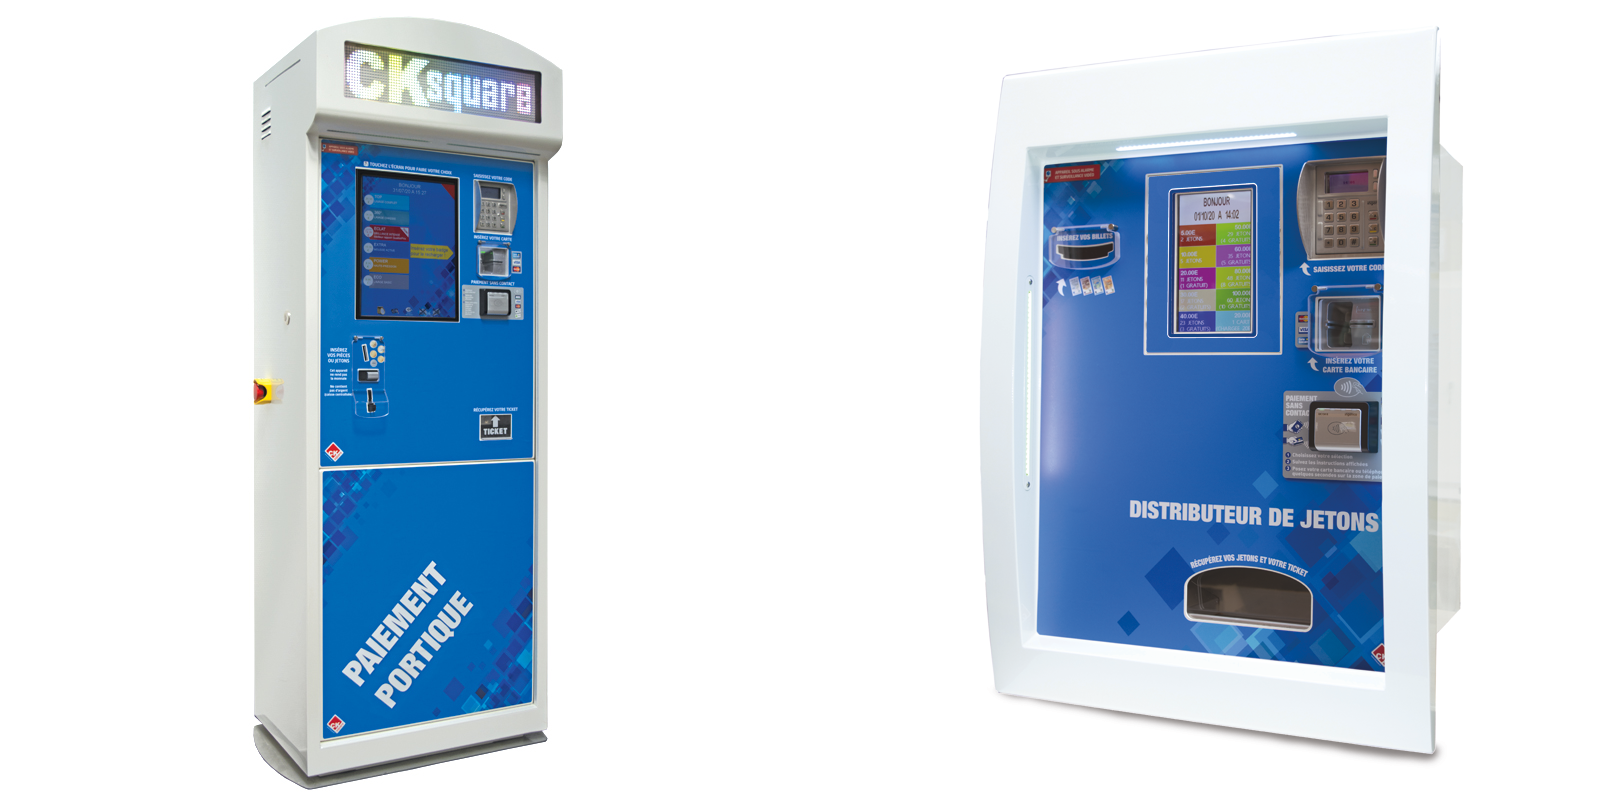
\includegraphics[scale=0.2]{./img/bornes.png}
  \caption{Produits CKsquare}
    \label{bornes-intro}
  \end{center}
\end{figure}
%}}}

CKsquare fait partie du groupe le Petit Poucet (LPP) composé de cinq sociétés
qui travaillent en collaboration. Parmi ces entreprises, on compte la société
M-Innov qui se charge de la conception et de l'installation des bornes et
systèmes monétiques pour les aires de services, campings, parking ou hôtels. La
société Mecasystem International, elle, se charge de la tôlerie et de la
mécanique pour les bornes CKsquare et M-Innov. La société Ehrse, née au sein
même de CKsquare, se charge des tests, du prés-montage et du câblage des cartes
électroniques. Enfin, il y a la société Logawin, société fille de CKsquare qui
est une entreprise de développement informatique. La société Logawin est
composée de deux pôles, Logawin France basé à Clermont-Ferrand et Logawin
Tunisie basé à Tunis. Ces cinq sociétés travaillent en coopération ce qui permet
au groupe CKsquare d'avoir la maitrise de la conception et de la fabrication de
tous les composants des produits. On peut voir sur la figure \ref{lpp-logos} les
logos des sociétés citées précédemment.

\clearpage

% [logos LPP] {{{
\begin{figure}[h!]
  \begin{center}
  
\includegraphics[scale=0.4]{./img/lpp-logos.png}
  \caption{Logos des membres du groupe LPP}
    \label{lpp-logos}
  \end{center}
\end{figure}
%}}}

L'objectif de la société CKsquare est de pouvoir fournir des produits
configurables et adaptables aux besoins des différents clients. C'est pour cela
que les bornes possèdent beaucoup d'options et que l'entreprise entretient un
savoir faire quant à la gestion de la plupart des systèmes de paiements
disponibles sur le marché. De plus, une équipe SAV reste à l'écoute du besoin
des clients ce qui permet à l'entreprise de concevoir des solutions encore plus
spécifiques et personnalisées.

Un des gros atouts de la société est son savoir faire concernant l'utilisation
des cartes électroniques. En effet, presque toutes bornes CKsquare sont équipées
de cartes électroniques beaucoup plus fiables et moins énergivores que des PC.
Cependant, ces cartes doivent assurer beaucoup de fonctionnalités et gérer un
grand nombre de composants ce qui pose de gros problèmes en terme d'optimisation
du stockage. En plus, la gestion de systèmes de paiements bancaires implique
encore plus de contraintes. Par exemple, la loi finance de 2016 (appliquée en
2018) a imposer la collection et la sauvegarde sécurisée des historiques de
paiement.
%}}}
\section{Travail demandé}%{{{

% TODO: faire un condencé de tout ça

% note: pas clair ici permettent d'interagir avec. Il faudra aussi des qui

L'objectif est de réaliser un outil servant à faire de l'intégration continue
pour valider les fichiers de la partie commune du code utilisé sur les bornes.
L'outil doit permettre l'écriture de tests pour valider le code et doit pouvoir
être automatisé dans une pipeline Gitlab. De plus, l'outil sera utilisé pour
tester du code exécuté sur du matériel embarqué, il faudra donc un moyen de
tester des fonctions qui interagissent avec le matériel électronique. Pour ce
faire, il faudra émuler les interactions avec le matériel en créant des
fonctions et des structures de données qui réagiront comme les composants
électroniques. Par exemple, si une fonction doit modifier un registre sur une
carte, il faut pouvoir émuler le registre pour vérifier que les bonnes
modifications ont été apportées dessus. Il faudra aussi des fonctionnalités
permettant de simuler l'interaction d'un utilisateur avec un composant pendant
les tests. Par exemple, on doit pouvoir faire en sorte de tester le comportement
du système lorsqu'un utilisateur appuie sur une séquence de touches. Il sera
donc nécessaire d'émuler la mémoire des composants électroniques, les fonctions
permettant de simuler les actions d'un utilisateur et les interfaces des
composants en utilisant divers protocoles de communication comme l'I²C et le SPI
mais aussi le Cctalk et le MDB.

Étant donné que les tests seront exécutés dans une pipeline (donc dans un
docker), il faudra s'assurer que le code puisse compiler sous Linux. De plus,
pour que le code fonctionne dans la pipeline, il faudra compiler avec gcc ce qui
nécessitera de remplacer une partie des bibliothèques de la carte, faites pour
être compilées avec le compilateur fourni avec MPLAB.

La première tâche sera de trouver le framework de test adapté pour la conception
de l'outil. Le code à tester est écrit en C, cependant, la société souhaiterait
aussi pouvoir tester les bibliothèques écrites par l'équipe Qt. Il serait donc
intéressant que l'outil soit aussi adapté au C++.

% validé
Le résultat final doit être un outil qui doit pouvoir être facilement
réutilisable et adaptable. La documentation et la structure du code doit pouvoir
permettre d'aisément modifier ou copier les différents éléments. Par exemple, il
faudra que tous les composants simulés aient la même structure et que cette
structure soit suffisamment simple et générique pour pouvoir être copiée pour la
création d'un nouveau composant.

% validé
À noter que l'objectif du projet n'est pas d'écrire des tests.  Des tests ont
été écrits durant le projet mais ces derniers ont pour objectif de valider le
bon fonctionnement des composants simulés et non celui du code de la société.
Par contre, il faudra fournir une documentation complète décrivant comment
tester les programmes. Cette documentation devra présenter le framework de test
et décrire le fonctionnement des composants simulés ainsi que leur utilisation.
%}}}
\section{Environnement et outils à disposition}%{{{

Concernant les conditions de travail durant le stage il faut noter que ce projet
se réalisait seul. Cependant, les développeurs de CKsquare étaient présents pour
répondre aux différentes questions, guider le projet ou pour faire les choix
importants.

Le projet a été démaré de zéro, aucun projet de test similaire n'avait été
amorcé auparavant. Le travail a été réalisé entièrement en présentiel. De plus,
les stagiaires étaient tous conviés aux réunions qui permettent de faire le
point au niveau des équipes de développement. Dans ces réunion chaque
développeur parle pendant deux minutes du travail qu'il a réalisé et de ce qu'il
compte faire ensuite.

Quant au matériel, un bureau avec un PC sous Ubuntu a été mis à disposition. La
session sur le PC possédait les privilèges administrateur pour faciliter
l'installation des différents logiciels utilisés pour le développement
(compilateur, éditeur de texte, doxygen, ...). De plus, il a été fourni une
boite mail ainsi qu'un compte Gitlab. Un projet Gitlab a aussi été créé pour
permettre de tester les frameworks de test. Il a aussi servit à stocker les
notes prise sur le projet ainsi que la documentation. Enfin, la documentation
des différents éléments comme les protocoles (Cctalk, Mdb) était disponible à la
demande.
%}}}
\clearpage
%***************************************************************************}}}
% Réalisation et conception ************************************************{{{
\part{Réalisation et conception}

\section{Choix du framework de test}%{{{

Le but du projet est de concevoir un outil permettant de tester du code, la
première tâche à donc été de choisir un framework de test. Le framework de test
constitue la base de l'outil, c'est donc un choix assez important. Dans cette
partie nous traiterons de la procédure qui a été utilisée pour trouver et
comparer des frameworks et des bibliothèques de test.

\subsection{Les critères de comparaison}%{{{

Étant donné le fait que le langage C est très utilisé, il y a beaucoup de choix
quand aux différentes bibliothèques de test utilisables. Le premier travail a
été de comparer bibliothèques et frameworks de tests existants. Une liste des
frameworks disponibles sur Wikipédia \cite{enwikiframeworks} a permis de prendre
connaissance des frameworks disponibles pour ensuite pouvoir faire plus de
recherches. Ce travail de recherche à permis de faire un prés tri et d'éliminer
les framework incomplets ou trop peu utilisés. Une fois la liste des meilleurs
frameworks terminée, il a fallut trouver des critères pour comparer les
frameworks. \\

Tout d'abord, l'équipe de développement souhaitait pouvoir tester à la fois du
code \textbf{C} et du code \textbf{C++} pour certaines parties développées par
l'équipe \textbf{Qt}. Ce critère était optionnel mais apprécié. À noter que
lorsque l'on parle de pouvoir tester du code C++, cela ne prend pas seulement en
compte le fait de pouvoir exécuter des fonctions basiques puisque c'est possible
avec tous les frameworks C étant donné la compatibilité entre le C et le C++.
Pour pouvoir tester du code C++, il faut aussi que le framework soit capable
d'interagir avec les structures de donnés fournis par la bibliothèque standard
de C++ ou encore de pouvoir traiter des exceptions. Étant donné ce critère,
l'idée d'utiliser un framework écrit en C++ a été envisagé.

Un autre critère concerne la modernité et la facilité d'utilisation du
framework. Cela peut sembler anodin mais l'écriture des tests est une tâche
aussi longue que le développement. Pour ne pas perdre de temps, il est
préférable que les tests soient le plus simple possible à mettre en place. De
plus, les tests peuvent aussi servir de documentation, c'est donc un avantage
non négligeable que d'avoir un framework qui permette d'écrire des tests
simples, lisibles et compréhensibles. Enfin, ce critère impacte aussi le temps
de conception de l'outil de test car le fait d'utiliser un framework trop
complexe aurait nécessité la conception de fonctions et macros (pour réduire la
complexité) et rallongé le temps d'écriture de la documentation. À noter que
pour valider ce critère, la documentation des différents outils a aussi été
étudiée, les frameworks devaient donc fournir une documentation suffisamment
claire et précise permettant d'utiliser facilement toutes les fonctionnalités
proposées.

% TODO: reformuler
Le critère le plus important est celui du statut du développement du framework.
En effet, lorsque l'on souhaite utiliser un outil, une question importante à se
poser est de savoir ce que l'on peut faire en cas de problème. Ici, il a fallut
regarder la taille, la popularité et l'age des projets. En effet, plus un projet
est populaire plus il sera facile de trouver de l'aide en cas de problème. De
plus, les projet important ont souvent beaucoup plus de collaborateurs ce qui
peut accélérer la corrections des bugs ou la vitesse de réponse au issue. Enfin
la dates de dernières mis à jours ont aussi été répertoriées car là aussi, il
est beaucoup plus simple de résoudre les problèmes sur un projet qui est encore
activement maintenu.

% TODO: mal dit
D'autres critères ont permis de démarquer les frameworks comme par exemple le
fait que les frameworks fournissent des fonctionnalités supplémentaires comme
l'export des résultats des tests dans différents format comme TAP ou XML (utile
pour faire des rapports) ou encore des générateur de nombres pseudo aléatoires
pour faire des tests avec des entrée aléatoires, \dots Une autre fonctionnalité
intéressante est que les frameworks exécutent les tests dans des threads séparer
ce qui permet de tester des signaux ou encore de ne pas stopper tous les tests à
cause d'une sortie erreur. Le fait que les frameworks utilisent beaucoup de
macros à aussi été pris en compte car bien que ces dernières permettent de
rendre le code beaucoup plus simple, elles peuvent aussi être source de
problèmes (elles ont parfois un comportement non souhaité et elles sont très
compliqué à déboguer). Le frameworks qui a été choisi possède ce défaut et nous
verrons les problème que cela pose lorsque nous détaillerons ce framework.
%}}}
\subsection{Les frameworks}%{{{

Dans cette section, nous allons faire une revue de tous les frameworks de tests
étudiés pendant le début du stage. Une fois ceci fait, nous présenterons le
choix final.

\subsubsection*{Check}

Le premier framework de la liste est Check, il propose un interface simple pour
l'écriture des tests, cependant, toute la mise en place des suites de tests est
plus complexe mais peut être changée facilement. Check permet d'exécuter les
tests dans des zones mémoires séparées ce qui permet de ne pas s'arrêter lors de
l'émission d'un signal comme SIGSEV. La bibliothèque Check est disponible avec
un paquet aptitude, ce qui le rend simple à installer. C'est aussi une bonne
preuve de la popularité de cette bibliothèque. Check est assez complet et donne
un rapport clair et facile à utiliser après l'exécution des tests. Le framework
permet de construire une structure de tests classique où l'on groupe les tests
dans des suites. Par contre, Check n'est pas compatible avec le C++.

Pour présenter les framework aux développeurs de la société, des exemples de
codes ont été présentés pour permettre d'avoir une idée de comment le framework
s'utilise. Sur le listing \ref{check-example} de l'annexe
\ref{appendix:frameworks-code} on peut voir un exemple d'utilisation de Check.

\subsubsection*{CUnit}

Le second framework est CUnit, il est aussi disponible avec un paquet aptitude
cependant. Le frameworks est assez complet et fourni beaucoup de fonctions
d'assertion. CUnit permet de construire la même structure de tests que Check, et
utilise des pointeurs de fonctions pour construire les suites. Pour chaque suite
de tests, on peut fournir deux fonctions qui seront exécutées avant et après les
tests pour permettre d'initialiser l'environnement de tests (ces fonctions sont
généralement appelées \textbf{setup} et \textbf{teardown}). Ce framework ne sera
pas compatible avec C++. Le framework CCPUnit est similaire à CUnit et permet
aussi de tester du code C, cependant, il est nécessaire d'utiliser des classes
C++ ce qui rend les tests plus complexes à mettre en place.

On peut voir sur le listing \ref{cunit-example} de l'annexe
\ref{appendix:frameworks-code} un extrait de code utilisant CUnit.

\subsubsection*{Criterion}

Le framework suivant est Criterion qui est assez récent et aussi disponible avec
un paquet aptitude. Il propose une interface très simple pour écrire des tests
et des suites de tests. On peut facilement ajouter les fonctions de setup et
teardown (pour les tests et les suites de tests) et les tests peuvent êtres
paramétrés. Comme Check, les tests sont exécutés dans des zones mémoires
séparées. On peut aussi facilement tester si un signal (comme SIGSEV) est émis
ou pas. De plus, le framework propose beaucoup de macros permettant de faire des
assertions non seulement sur les types primitifs, mais aussi sur les tableaux.
Enfin, Criterion possède aussi une interface C++.

À noter tout de même que la simplicité de l'interface de Criterion vient du fait
que le frameworks utilise beaucoup les macros ce qui peut poser problème.

On peut voir sur le listing \ref{criterion-example} de l'annexe
\ref{appendix:frameworks-code} un example de tests écrits avec Criterion.

\subsubsection*{Minunit}

Minunit est la plus simple des bibliothèques de tests trouvée. Elle ne se
compose que d'un fichier d'entête. L'interface proposée est très simple mais
très basique, elle permet seulement l'écriture de tests et de suites de tests.
Cette bibliothèque est une collections de macros qui pourraient être utilisées
pour créer un framework de test plus complet. La bibliothèque fourni aussi
quelque fonctions d'assertion.

On peut voir sur le listing \ref{minunit-example} de l'annexe
\ref{appendix:frameworks-code} un exemple d'utilisation de Minunit.

\subsubsection*{Munit}

Munit propose une interface plus complexe car cela nécessite d'utiliser des
tableaux et des structures. Pour les tests, les fonctions de tests sont très
simple à écrire et il y a la possibilités d'avoir différents types de retours.
Pour chaque test, on peut associer les fonctions de setup et de teardown. Les
tests peuvent aussi être paramétrés. Le framework propose aussi une interface en
ligne de commande, il est donc possible de donner des paramètres au programme
pour choisir quels tests sont exécutés. Il est aussi possible de construire une
structure de test plus complexe cas on peut avoir des suites de suites de tests.
Le framework propose aussi des fonctions de génération de nombres aléatoires.

On peut voir sur le listing \ref{munit-example} de l'annexe
\ref{appendix:frameworks-code} comment s'utilise Munit.

\subsubsection*{Unity}

Framework de test spécialisé pour les systèmes embarqué, léger et simple. Il ne
permet pas de construire une structure de tests très complexe (seulement de
simple tests) mais possède beaucoup de fonctions d'assertion. En terme
d'interface, le framework propose une collection de macros simples et lisibles.
Le framework fourni aussi un script pour faciliter la mise en place des tests
(en revanche ce script est assez mauvais car il ne génère un runner que pour une
seule suite).

Le framework possède beaucoup de fonctions d'assertions mais il ne possède pas
beaucoup plus de fonctionnalités. Il ne sera pas utilisable pour tester du code
qui utilise des fonctionnalités propres à c++ comme les exceptions par exemple.

On peut voir sur le listing \ref{unity-example} de l'annexe
\ref{appendix:frameworks-code} un exemple de test utilisant Unity.

\subsubsection*{Tau}

Très léger, le framework ne se compose que de fichiers d'entête. Il permet de
construire une structure de tests avec des tests et des suites de tests. Les
tests sont écrits en utilisant des macros, ce qui rend l'interface très simple.
Tau permet facilement d'avoir plusieurs fichiers de tests en générant son propre
main. Par contre, il ne permettra pas de tester les exceptions en C++.

On peut voir sur le listing \ref{tau-example} de l'annexe
\ref{appendix:frameworks-code} un extrait de code utilisant Tau.
%}}}
\subsection{Le choix final}%{{{

Le choix final s'est porté sur Criterion car le framework possède beaucoup
d'avantage. Tout d'abord, il est le seul à être complètement compatible avec le
C++ et ce, sans proposer une interface nécessitant la mise en place de classe
comme ce que l'on pourrais voir avec CPPUnit. De plus, ce framework est très
simple d'utilisation, il permet d'écrire des tests clairs facilement et
rapidement. Il propose aussi beaucoup de fonctionnalités comme la possibilité de
générer des logs, les tests paramétrés, les théories (tests des vecteurs
d'entrées et de sorties) et possède aussi une interface en ligne de commande
permettant de passer des options en paramètres du programme.

Par contre, la simplicité d'utilisation de ce framework cache une grande
complexité au niveau de son implémentation. Le framework a posé quelques
problèmes mineurs dans la suite du projet. Tout d'abord, la simulation des
composant nécessite l'appel de fonctions d'initialisation au préalable et cela
aurait été pratique de le faire dans la fonction \lstinline{main}. Comme
expliqué dans les parties précédentes, le framework génère son propre point
d'entré, cependant il est possible d'écrire la fonction \lstinline{main} à la
main si besoin. Le problème est que pour une raison inconnue, cela n'a pas
marché lors des essais au début du projet (d'après le message d'erreur, le
problème venait des threads). Ce n'est pas un problème grave car Criterion
propose beaucoup d'outils qui permettent de mettre en place des solutions
alternatives mais c'est tout de même un point important à noter. De plus, le
fait que le framework utilise beaucoup de macros pose parfois problème car ces
dernière peuvent avoir des comportements indésirables. Par exemple, il peut
arriver qu'un test basique d'égalité avec la fonction d'assertion principale ne
compile plus lorsque l'on échange les expressions de par et d'autre de
l'opérateur \lstinline{==}. Les macros peuvent être très utiles et très
puissantes, elles permettent ici de rendre le code beaucoup plus lisible,
cependant, il faut noter que les macros trop complexe sont très difficiles à
écrire et à déboguer.

Le framework choisit possède donc beaucoup de qualité mais aussi quelques
défauts. Au final, bien que ce framework ne soit pas parfait, il remplit
bien son rôle et il propose beaucoup de fonctionnalités très utiles pour
écrire les tests. De plus, il faut noter que ce framework est assez récent, il
est donc normal qu'il y ai encore des défaut qui seront certainement corrigés
au fil des années de développement.
%}}}
%}}}
\section{Organisation d'un projet CKsquare}%{{{

L'outil créé pendant ce stage a été testé sur un projet de l'entreprise. Cela a
permis dans un premier temps de pouvoir voir et comprendre comment le code à
tester fonctionne puis ensuite cela à permet de vérifier la bonne intégration de
l'outil dans le projet. Dans cette partie, nous détaillerons comment sont
organisés les projets de CKsquare. Cela permettra une meilleur compréhension des
choix qui ont été fait par la suite.

\subsection{Organisation des fichiers}
\label{orgaprojck}

Dans cette partie, nous allons détailler comment sont organisés les fichiers
dans un projet CKsquare puis nous traiterons le fonctionnement du code dans la
partie suivante. On rappel que ce projet d'intégration continue ne concerne que
la partie du code qui est commune à tous les projet et qui est incluse sous la
forme d'un sous module git. \\

Pour pouvoir penser le fonctionnement de l'outil de test à créer pendant ce
stage, il était important de comprendre le fonctionnement général du projet.
Avant de s'intéresser au fonctionnement, il faut comprendre comment le code est
organisé. Cela permet deux choses, premièrement, cela permet de ne pas se perdre
et de pouvoir facilement retrouver les fichiers. Pour comprendre le
fonctionnement du code, il est important d'avoir un plan de l'organisation.
Deuxièmement, il est aussi très important de comprendre comment s'est organisée
l'entreprise pour pouvoir organiser le code de l'outil créé. En
effet, l'organisation du projet de test doit suivre les principes de CKsquare
pour rendre l'outil facile à utiliser et à maintenir pour les développeurs de
l'entreprise.

%TODO: glossaire PIC
%TODO: dire que la config = challenge
Sans s'attarder trop sur les détails, l'organisation d'un projet est la
suivante. Chaque projet comporte une partie locale dans laquelle, tous les noms
de fichiers commencent par un \textbf{l}. Dans cette partie, on retrouve trois
fichiers principaux. Tout d'abord, il y a le fichier \lstinline{linit.c} qui
permet d'initialiser le projet. Ensuite, il y a les fichiers \lstinline{lmain.c}
et \lstinline{lloop.c} qui permettent de gérer la fonction \lstinline{main} et
la boucle principale du projet. Le projet local contient aussi deux fichiers
très importants car ils permettent de configurer le projet. Ces fichiers se
nomment \lstinline{config.h} et \lstinline{config_hw_default.h}. Ce sont des
fichiers d'entête à l'intérieur desquels sont définis des constantes
préprocesseur. Les projet CKsquare fonctionnent beaucoup sur le principe de la
compilation conditionnelle. Les constantes préprocesseurs sont gérées à la
compilation pour inclure ou non des parties du code, ce qui permet d'ajouter ou
d'enlever facilement des fonctionnalité. Lorsqu'une fonctionnalité est enlevée,
elle n'est pas compilée et le code correspondant n'apparait pas dans
l'exécutable. De ce fait, il n'impacte pas sa taille, ce qui est très
intéressant du fait des limitations quand aux capacités de stockage sur les
carte. Nous verrons dans les parties suivantes l'importance de ces configuration
pour compiler les fichier et aussi pour tester les différentes parties du
projet. Chaque projet contient aussi un répertoire \lstinline{CKLibs} dans
lequel se trouvent des \gls{smodg}. Sur le projet d'étude qui a permis la mise
en place du projet de test, il y avait deux sous modules. Le premier sous module
se nomme \lstinline{commun_global} et il contient la partie du code qui est
commune à tous les projet C \textbf{et} C++. Le second sous module est
\lstinline{dev_pic} et comme son nom l'indique, ce dernier ne concerne que la
partie C qui s'exécute sur un \gls{pic}.

La partie que nous allons traiter se trouve dans le répertoire
\lstinline{dev_pic}. Ce répertoire contient un sous répertoire
\lstinline{commun} qui contient la partie du code à tester. Le sous répertoire
\lstinline{commun} n'est pas la seule chose intéressante dans
\lstinline{dev_pic} puisque ce dossier contient aussi les bibliothèques des
différents compilateurs. L'entreprise CKsquare a réécrit une grande partie des
bibliothèques des \gls{pic}s pour avoir plus de maitrise quand à la gestion des
différents éléments. Ces bibliothèques ont été très utiles pour mettre en place
une partie de l'émulation des composants dans le projet de test, nous traiterons
cela plus loin dans ce rapport. Le reste des bibliothèques des microcontrôleurs
a aussi été utilisé pour compiler avec gcc, là aussi, ce sera traiter dans les
prochaines sections.

Le code commun est organisé par catégories. Le répertoire \lstinline{commun} de
\lstinline{dev_pic} contient des sous répertoires qui correspondent au
catégories. Par exemple, on retrouve le dossier \lstinline{StorageDriver} qui
contient les fichiers qui gèrent le stockage ou encore le dossier
\lstinline{Payment} qui contient tous ce qui concerne le paiement (types de
paiement, accepteur de pièce, \dots). L'objectif est de pouvoir faire des
recherche par catégories et de garder les dépendance au plus proche des
fichiers. Par exemple, plusieurs des sous répertoires de \lstinline{commun}
contiennent un dossier \lstinline{Web} qui regroupe les dépendances web des
fichiers de chaque catégories. On peut ainsi retrouver facilement les dépendance
des fichiers.

Pour résumer, les projets CKsquare sont composés d'une partie locale, spécifique
au projet. Parmi ces fichier locaux, on retrouve le fichier responsable de
l'initialisation, le point d'entrée, la boucle principale ainsi que la
configuration du projet. Les projets incluent des bibliothèques sous la forme de
\gls{smodg} stockées dans le répertoire \lstinline{CKLibs}. Parmi ces
bibliothèques on retrouve le projet \lstinline{dev_pic} qui contient le code
commun à la partie C qui s'exécute sur les cartes électroniques de l'entreprise,
et c'est ce code que l'outil créé durant ce stage va testé. À noter qu'ici, on
ne s'intéresse qu'à l'essentiel pour permettre une explication rapide du
fonctionnement général du projet dans la partie suivante. Cependant, le projet
comporte beaucoup d'autre fichiers qui ne sont pas décrit dans ce rapport.\\

Maintenant que nous avons expliqué l'organisation générale du projet, nous
allons pouvoir traiter le fonctionnement de ce dernier.

\subsection{Fonctionnement du projet}

Résumé synthétique du fonctionnement global du code.

TODO: Le code de CKsquare utilise principalement des machines à états...

Machines à état: contraintes => pas accès aux états dans les tests
\cite{teststatemachines}.
%}}}
\section{Organisation du projet de tests}%{{{

Dans cette partie, nous allons détailler la structure du projet de test. Cette
structure s'appuie sur celle des projets de l'entreprise.

Il est important de noter que l'organisation du projet de test à changée. Au
départ, le projet de test devait être un projet à part. Ce dernier devait être
cloné dans pipeline du projet \lstinline{dev_pic} pour pouvoir tester les
fichiers. Au final, il a été décidé d'intégrer complètement le projet de test
dans \lstinline{dev_pic}. L'organisation des tests suis les principes expliqués
dans la section \cite{orgaprojck}. De ce fait, les tests sont stocké à proximité
des fichiers testés.

\subsection{Faux projet et gcc}

TODO: détail de \lstinline{FakeProject} et \lstinline{gcc}.

\subsection{Les versions test}

TODO: détail de \lstinline{TestLibraries}.\\
TODO: détail de la création d'une version test (reprendre la doc d'IOS)

\subsection{L'émulation}

TODO: détail de \lstinline{Emulation}.

\subsection{Le répertoire Test principal}

\subsubsection{Configuration de Criterion}
\label{configuration-de-criterion}

\subsection{Les tests}

TODO: détail de \lstinline{tests}.

\subsection{Cmake}

Dans cette partie nous allons voir comment est compilé le projet de test. Nous
justifierons tout d'abord le choix de l'utilisation de CMake. Ensuite, nous
détaillerons l'organisation et le fonctionnement de la configuration de cet
outil.

Au début du projet, l'outil choisit pour compiler était Makefile. L'avantage de
Makefile est qu'il est assez proche du script, ce qui donne une grande
flexibilité car on défini toutes les commandes à la main. Le défaut de Makefile
est qu'il peut très vite devenir peu lisible. De plus, sur de gros projet, mettre
en place de la compilation séparée peut être très complexe, or cela était
nécessaire pour le développement du projet étant donnée le nombre de fichier à
compiler. L'outil de test à créer devait être suffisamment simple à utiliser et à
modifier, la complexité croissante du Makefile à mesure que le projet avançait a
pousser à l'utilisation de CMake.

CMake est un outil qui permet de générer un Makefile très complexe. Il permet de
mettre en place de la compilation séparée sur de gros projets automatiquement.
La configuration de CMake est assez simple et beaucoup plus lisible que celle de
Makefile. De plus, CMake propose des fonctionnalités avancées comme la gestion
automatique des bibliothèque ou encore \textbf{CTest}, qui permet d'automatiser
l'exécution de tests. Détaillons à présent la configuration de cet outil.

Le fichier de configuration de CMake est le fichier \lstinline{CMakeLists.txt}
(il doit avoir exactement ce nom). Il faut un ficher de configuration par sous
projet. Ici, il n'y a que le projet de tests alors ce fichier se trouve dans le
répertoire \lstinline{commun/Tests}.

La configuration comporte les six sections suivantes:

\begin{itemize}
  \item \textbf{configuration du projet}: cette partie contient la configuration
    minimale de CMake. Ici, on spécifie la version minimale de CMake requise
    ainsi que le nom du projet. Cette partie comprend aussi l'ajout du framework
    Criterion à l'édition des liens ainsi que des options pour \lstinline{gcc}
    comme l'option \lstinline{-g} par exemple (débogage avec gdb).
  \item \textbf{jeux de tests}: dans cette partie, il y a plusieurs listes de
    fichiers tests (stockées dans des variables réutilisables plus loin). Il y a
    plusieurs jeux de tests car on souhaite générer plusieurs exécutables. Comme
    dit précédemment, il y a plusieurs configurations du projet à tester. Chaque
    exécutable correspond à une fonctionnalité qui nécessite une configuration
    particulière.
  \item \textbf{projet de test}: cette partie contient la liste des fichiers
    relatifs au projet de test.
  \item \textbf{projet commun}: ici on a une liste qui contient les fichiers du
    projet \lstinline{dev_pic} qui sont à compilés avec tous les exécutables. Ce
    sont les fichiers dont tous les jeux de tests ont besoin.
  \item \textbf{exécutables}: dans cette partie, on génère les exécutables en
    spécifiant les bonnes listes de fichiers à compiler. De plus, pour chaque
    exécutable, on utilise une commande CMake qui permet de définir des
    constantes préprocesseur lors de la compilation (option \lstinline{-D} de
    gcc). Cela permet de choisir les configurations du projet pour les tests.
  \item \textbf{tests}: dans cette section, on ajoute les exécutables à la liste
    des tests. Ces tests pourront être lancé par \lstinline{CTest} après la
    compilation.
\end{itemize}

%TODO: conclusion cmake

%}}}
\section{Simulation des horloges}%{{{

Le premier élément qui a été simulé était l'horloge principale du programme. Par
la suite, c'est l'horloge Rtc qui a été simulée en suivant le même principe que
pour l'horloge principale. Dans cette section nous allons traiter le
fonctionnement de ces composants.\\

Au début du projet, quelques tests simples ont été réalisés sur certains
fichiers, cependant, il est rapidement devenu évident que certaines fonctions
n'allaient pas pouvoir être testées à cause de l'horloge. En effet, à plusieurs
endroits dans le code, on met en place des temps d'attente et le programme est
bloqué tant que le temps d'attente n'est pas passé. L'horloge est gérée dans le
code à travers une variable globale \lstinline{TIMER_Centieme} et cette dernière
doit être incrémentée pour que le temps passe. Dans le cas contraire, le
programme reste bloqué.

Le problème technique que pose la simulation des horloges est qu'il faut que ces
dernières fonctionnent en même temps que le programme principale tourne.
L'implémentation la plus simple consiste à incrémenter les variables d'horloge
dans les tests à chaque fois que l'on sait qu'un temps d'attente est mis en
place. Cette solution n'était pas suffisamment pratique et réaliste. Pour ce
problème, il a été très rapidement décidé d'utiliser des threads. L'objectif
était d'incrémenter les variables des horloges dans des fonctions simples
s'exécutant dans un processus séparé en même temps que le programme principal.

Cette solution a été très simple et rapide à mettre en place étant donné que les
processus n'avaient pas besoin d'être synchronies. Au final, les deux horloges
fonctionnent sur le même principe. Pour chacun des fichiers on a une fonction
\lstinline{Start} qui permet de créer le thread. Cette fonction possède une
sécurité qui fait que l'on peut faire autant d'appels que l'on souhaite, le
thread n'est créé qu'une seule fois (cela rend l'utilisation plus simple dans
les tests). À noter que dans le cas du Rtc, l'horloge démarre à la date du jour.
Les fichier comportent aussi une fonction \lstinline{Loop} qui est la fonction
qui s'exécute dans le thread. De plus, des moyen d'interagir avec les horloges
ont étaient ajoutés. Par exemple, à certains endroits du code, on met en place
des temps d'attente relativement long. Pour éviter de bloquer le programme,
chaque fichier propose une fonction \lstinline{Wait} qui permet d'incrémenter le
compteur manuellement. Il est aussi possible de mettre les horloges en pause et
de les relancer. Enfin, il y a une fonction \lstinline{Stop} qui permet de
détruire les threads. Les fonctions \lstinline{Start} et \lstinline{Stop} sont
appelées dans les fonctions d'initialisation et de terminaison globales décrites
dans la section \ref{configuration-de-criterion}.\\

Les horloges représentaient donc une partie importante du projet car elles sont
énormément utilisées dans le code et si les compteurs ne sont pas incrémentés,
il devient impossible de tester les fonctions. La solution qui a été trouvée est
très simple et assez réaliste en plus d'être assez pratique à utiliser dans les
tests. Dans la section suivante, nous traiterons le deuxième éléments qui a été
simulé lors de la création de l'outil de test et qui propose une solution
différente de celle utilisée avec les horloges.
%}}}
\section{Simulation du stockage}%{{{

Une partie importante de l'émulation concerne le stockage et il y a plusieurs
types composants à simuler, les registres, les eeproms, et la mémoire flash.
L'émulation des périphériques des stockage est assez simple puisqu'il s'agit
simplement de tableaux de caractères non signés (codés sur 8 bits sur la plupart
des machines). La partie complexe de l'émulation du stockage concerne
l'interface qui permet d'interagir avec les périphériques. Il y a deux
protocoles qui sont utilisés avec le stockage. Tout d'abord il y a le protocole
I²C qui est utilisé avec les registres et certaines eeproms. Ensuite il y a le
protocole SPI qui est utilisé avec les eeproms et les mémoires flash.

Dans cette partie nous allons voir comment a été réalisée l'émulation de
l'interface permettant d'utiliser le stockage avec les différents protocoles.

\subsection{Échec des threads}

La première solution qui a été implémentée utilisait des \textbf{threads} de la
même façon que les horloges. L'objectif été de pouvoir simuler les composants de
sorte à ce qu'ils se comportent comme les composants réels installés sur la
carte. Pour se faire, il été souhaitable que les composants simulés soient actif
en même temps que la carte (représentée ici par le programme à tester) et c'est
pour cela que les threads ont été utilisés. Le principe était que les composants
étaient représentés par des machines à états qui bouclaient dans un état de base
jusqu'à ce que le composant soit appelé (donc jusqu'à ce que le programme
principale décide de lancer une communication en utilisant un des protocoles
cités précédemment). Une fois le composant appelé, la machine à états permettait
d'assurer la communication. Pour que les composants simulés s'exécutent en même
temps que le programme principale, ils s'exécutaient dans des threads séparés.
\\

Le problème des threads réside dans la synchronisation de ces derniers. Il y a
différentes méthodes pour synchroniser des threads. Sur ce projet, il a au
départ été utiliser des boucles infinies qui permettait de faire attendre les
threads. Par exemple, le programme principale était stoppé par une boucle pour
attendre que le les composants émulés s'exécutent et le débloque. Cette solution
a été utilisée au départ car ce genre de boucles été déjà présentes dans
l'implémentation de l'I²C. Par la suite, cette solution s'est avérée complexe
d'utilisation et peu élégante, les boucles ont donc étaient remplacées par des % todo: expliquer les sémaphores
sémaphores. Au final, la synchronisation des threads est devenue trop compliquée
et très peu fiable (l'exécution du programme ne donnait pas toujours les même
résultats). L'objectif du projet étant de concevoir un outil qui soit facilement
réutilisable, cette solution était trop complexe et donc pas adaptée. Il a donc
été décidé de ne plus les utiliser les threads même si la nouvelle solution
devait être moins pratique d'utilisation au niveau de l'écriture des tests.

\subsection{Interface I²C}

Dans cette partie, nous allons voir le fonctionnement de l'émulation de
l'interface I²C du stockage. Nous commencerons par voir les principes du
protocole I²C puis nous détaillerons le fonctionnement de la simulation.

\subsubsection*{Le protocole I²C}

TODO: protocole \cite{mankar2014review}
TODO: parler des fichiers

\subsubsection*{Émulation}

TODO: comment fonctionne la simulation de l'I²C

\subsection{Interface SPI}

Le second protocole utilisé avec le stockage est le protocole SPI. Comme pour le
protocole I²C traité dans la partie précédente, nous commencerons par expliquer
le fonctionnement du protocole puis nous détaillerons l'émulation.

\subsubsection*{Le protocole SPI}

TODO: \cite{dhaker2018introduction} et \cite{li2014design}

\subsubsection*{Émulation}

TODO: comment fonctionne l'émulation du SPI

\subsection{Système d'évènements}

TODO: explication du système d'évènement qui permet de vérifier le respect du
protocole et la bonne utilisation des fonctions bas niveau.
%}}}
\section{Les interfaces des composant}%{{{

\subsection{L'interface Cctalk}%{{{

Une partie des composants utilisé sur la carte ont été interfacés avec le
protocole Cctalk. Dans cette section, nous commencerons par détailler les grands
principes de ce protocole puis nous verrons l'implémentation du protocole par
l'entreprise. Enfin, nous expliquerons comment les périphériques Cctalk ont été
simulés.

\subsubsection{Le protocole}

TODO: explication rapide du protocole

La documentation est en 3 parties:
- \cite{cctalkpt1}: présentation du protocole \\
- \cite{cctalkpt2}: headers \\
- \cite{cctalkpt3}: commandes

\subsubsection{Le code de l'entreprise}

TODO: détail du fonctionnement du code de l'entreprise (modélisation des
commandes, les fichier \lstinline{CctalkMaster.c} et
\lstinline{CctalkMasterSerial.c}).

\subsubsection{Émulation des composants}

TODO: 1 fichier par composant, trois fonctions (Control, Run et HandleResponse),
2 utilisations possibles, ...\\
TODO: parler de comment cette solution final à été trouvée et des premières
version créées (cf: notes week 9)\\

Émulation bas niveau:\\

TODO: Faite en premier car permettait de mieux comprendre le protocole et le
fonctionnement du code. De plus, c'est la partie la plus importante car elle
permet de tester tous les éléments du code ce qui n'est pas le cas de l'autre
version.\\

Émulation haut niveau\\

TODO: l'interface cctalk a été réécrite pour envoyer directement les réponse aux
commande dans une seconde version de la fonction CmdSnd ... (TestLibraries++)
%}}}
\subsection{L'interface MDB}%{{{

Dans la partie précédente nous avons traité le fonctionnement du protocole
Cctalk et nous avons aussi vu comment les composants Cctalk ont été simuler pour
faire fonctionner les tests. Dans cette partie, nous allons traiter un autre
protocole utilisé avec d'autre composants, le protocole MDB. Cette partie va
suivre un plan similaire à la précédente.

\subsubsection{Le protocole}

TODO: \cite{mdbdoc}

\subsubsection{Le code de l'entreprise}

\subsubsection{Émulation des composants}

\subsubsection{Système de scénarios}
%}}}
\subsection{L'interface TCPIP}%{{{

TODO: Il n'est pas certain que cette partie paresse dans le rapport final
%}}}
%}}}
\section{Les historiques}%{{{

Dans cette section, nous allons nous intéresser aux historiques. Les historiques
(de paiement, d'évènements) sont stockés dans une base de donnée circulaire.
C'est un élément important car la sauvegarde des historiques est juridiquement
obligatoire quand ils concernent la monétique. Dans cette partie, nous
commencerons, dans un premier temps, par détailler le fonction de la structure
de donnée et des tests qui ont été fait dessus. Dans un second temps, nous
traiterons le fonctionnement des historiques.

\subsection{Les CDBs}

Tous les historiques sont stockés dans un base de donnée circulaire (CDB
signifie \textit{Circular Data Base}). La première partie des tests concernant
les historiques va porté sur la validation du bon fonctionnement de cette
base. Un point important concernant cette structure est que les CDB sont stockées
en mémoire (généralement sur des eeproms). Les tests qui vont être réalisés sur
cette structure vont permettre de valider le fonctionnement de l'émulation du
stockage. De plus, ils vont constituer un exemple intéressant qui pourra être
décrit dans la documentation.

TODO: fonctionnement des CDB.\\
TODO: réutilisation du stockage.

\subsection{Tests des historiques}

TODO: pour conclure cette partie dire que c'est un problème avec les historiques
qui a donnée l'idée du stage à l'entreprise.
%}}}
\section{Mise en place de la pipeline}

\section{Déroulement du projet}

\subsection{Les outils utilisés}%{{{

Dans cette partie, nous allons faire une revue des outils utilisés pendant le
stage. Les outils les plus utilisés ne seront pas détaillé, par contre, cette
partie a pour but de mettre en lumière les avantages qu'il y a à connaitre et
configurer ses outils de travail.

\subsubsection{Gestion de version}

Pour la réalisation du projet, le gestionnaire de version utilisé été Git. À
noter que la société n'utilise Git que depuis un ans, le gestionnaire de version
qu'ils utilisaient avant été SVN.

L'avantage de Git est qu'il est assez simple d'utilisation mais propose tout de
même des fonctionnalités très complexes. De plus, par rapport à SVN, Git est
décentralisé et permet de faire des branches ce qui a été très utile pour éviter
que le projet de tests pose problème.

La philosophie de travail utilisé a consisté en une version réadapté de Gitflow.
Le principe de Gitflow est d'avoir une branche \lstinline{master} qui va
contenir les versions du projet. Ensuite, il y a une branche \lstinline{dev} qui
est utilisée pendant le développement. La branche \lstinline{dev} contient du
code fonctionnel mais qui n'est pas encore déployé sur \lstinline{master}. Entre
les branches \lstinline{master} et \lstinline{dev} il doit normalement y avoir
une branche \lstinline{release} qui contient des prés-versions mais elle n'a pas
été utile ici. Enfin, à partir de la branche \lstinline{dev}, on créer des
branches de \lstinline{features} sur lesquelles on développe les nouvelles
fonctionnalités. Étant donné que le travail se faisait seul, le fait d'utiliser
Gitflow avec autant de branche n'était pas vraiment nécessaire. Cependant, cette
méthode permet d'être très organisé. Cela permet par exemple de toujours avoir
du code fonctionnel présentable à un collègue. De plus, cette organisation des
branches permet de ne pas se perdre et de ne jamais caser du code fonctionnel.
L'avantage des branches est que l'on peut facilement faire des tests pour savoir
si une solution est réalisable.

À noter que l'équipe de développement de CKsquare utilise l'application
\textbf{gitahead}. Cette application n'a pas été utilisée pendant le
développement du projet de tests. C'est l'interface en ligne de commande de Git
qui a été privilégiée ainsi que l'utilisation du plugin \textbf{fugitive} sur
neovim.

\subsubsection{Doxygen}

TODO: Génération automatique de la documentation à partir des commentaires
laissés dans le code. Présentation rapide de doxygen

% \subsubsection{Compilation}

% L'objectif étant de pouvoir automatiser les tests dans une pipeline Gitlab, il
% fallait obligatoirement que les tests puissent compiler sur un docker et donc
% sur un Linux. L'outil le plus adapté pour ce genre de tache est
% \textbf{Makefile} qui a été utilisé en début de projet. Le défaut de Makefile
% est qu'il reste assez proche du script et qu'il faut obligatoirement détailler
% toutes les commandes. Étant donné le fait qu'il y avait beaucoup de fichiers, le
% Makefile est vite devenu très compliqué et illisible et ce même si aucune
% compilation séparé n'a été mise en place au début du projet. Quand de plus en
% plus de fichiers ont été ajoutés au projet de test, il a fallut mettre en place
% de la compilation séparée pour ne pas tout recompiler à chaque fois. Faire cela
% avec Makefile est tout à fait possible mais cela aurait pris beaucoup de temps     % rep cela
% et le fichier final aurait été assez peu lisible et surtout assez compliqué à
% comprendre. Le but étant de faire un outil facilement compréhensible et
% utilisable par tous les membres de l'entreprise, il fallait trouver une solution
% plus simple. La syntaxe de \textbf{CMake} à permis de simplement lister les
% fichiers à compiler ainsi que les répertoires à inclure sans avoir besoin de
% détailler les option de gcc. Cet outil permet de générer un Makefile complet
% avec un syntaxe beaucoup plus simple. De plus, CMake permet nativement de faire
% de la compilation séparer ce qui à permis de gagner du temps pendant le
% développement étant donner le fait que seuls les fichiers modifiés sont
% recompilés lors de l'écriture des tests.

\subsubsection{GDB}

TODO: Un des objectifs de ce stage été de progresser sur l'outil GDB.\\
TODO: utilisation avancée de gdb\\
TODO: configuration de gdb

\subsubsection{IDE}

TODO: nvim -> vim-fugitive, clangd, l'intégration de gdb ... Présentation rapide
de ma configuration.
%}}}
\subsection{Rédaction de la documentation}%{{{
\clearpage
%}}}
\subsection{Planification des tâches}%{{{

Les tâches prévues lors du stage étaient les suivantes. Au départ, il était
prévu de faire le choix du framework de tests puis de faire une revue des
éléments du code à tester. Ensuite, il était prévu de faire des tests sur des
fichiers simples pour s'habituer au code de l'entreprise et aussi permettre de
compiler une première partie du projet. Une fois le projet pris en mains,
l'objectif était de s'attaquer aux grandes parties qui étaient tout d'abord le
stockage, puis le Cctalk et le MDB. Les historiques devaient être testés à la
fin du fait de leur dépendance au stockage. Il était aussi prévu de réaliser de
la documentation en parallèle tout au long du projet.

% [expected gantt] {{{
\begin{figure}[h!]
  \begin{center}
  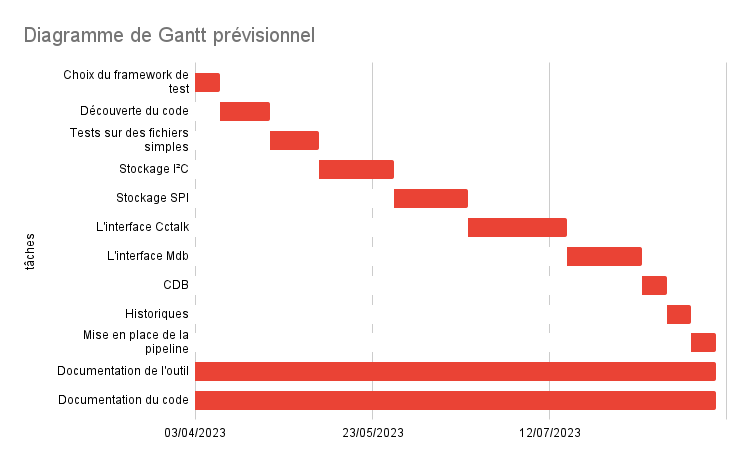
\includegraphics[scale=0.6]{./img/expected-gantt.png}
  \caption{Diagramme de Gantt prévisionnel}
  \end{center}
\end{figure}
%}}}

L'organisation de ces tâche a été faite sans connaissance de la complexité du
code. Certains des composants de l'outil final ont été refait plusieurs fois car
les résultats ne satisfaisaient pas les critère nécessaire à leur validation.
C'est le cas du stockage où au départ il avait été fait le choix d'utiliser des
threads, un choix qui a été remis en cause par la suite. Un autre exemple serait
celui du Cctalk dont certaines parties ont été réécrites suite à
l'implémentation de l'émulation des composants MDB pour ajouter plus de
cohérence. Malgré le fait que certains éléments ont été refaits, le
développement a pris moins de temps que prévu. Les tâches ont été surévaluées du
fait du manque de connaissances sur certains éléments comme les protocoles par
exemples.

NOTE: diagramme actuel

% [current gantt] {{{
\begin{figure}[h!]
  \begin{center}
  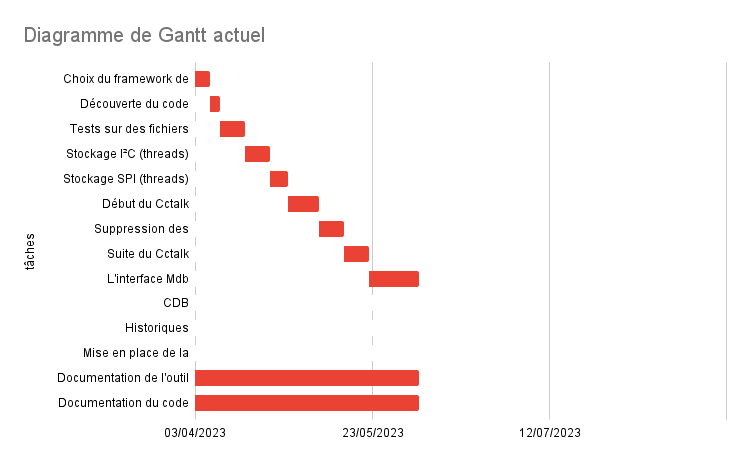
\includegraphics[scale=0.6]{./img/current-gantt.png}
  \caption{Diagramme de Gantt actuel.}
  \end{center}
\end{figure}~\\
%}}}
%}}}
\clearpage
%***************************************************************************}}}
% Résultats et discussions *************************************************{{{
\part{Résultats et discussions}

\section{L'outil final}

Description de l'outil final réalisé à la fin du stage.

TODO: Rétrospective sur le choix du framework (problème macros, ...).

\clearpage

\section{Discussion et perspectives}

Regard sur ce qui a été fait et comment cela a été fait (parler de l'échec
des threads, manque de bibliographie, ...). Parler de ce qui reste à faire ou a
améliorer.

\clearpage

\section{Développement durable}

NOTE: Je ne sais pas comment nommer cette partie, elle doit correspondre à la
réflexion sur les enjeux actuels liés à la responsabilité sociétale et
environnementale demandée par la CTI.

\clearpage

\section*{Conclusion}
\addcontentsline{toc}{section}{Conclusion}

CONCLUSION

%***************************************************************************}}}

%------------------------------------------------------------------------------%
%                                 bibliography                                 %
%------------------------------------------------------------------------------%

\section{Résumé biblio (WARN: section temporaire)}

Test affichage biblio:

\begin{itemize}
  \item \cite{enwikiframeworks}: liste des frameworks sur Wikipédia
  \item \cite{enwikifixtures}: définition fixture Wikipédia
  \item \cite{teststatemachines}: tester des machines à états
  \item \cite{mankar2014review}: présentation du protocole I²C
  \item \cite{dhaker2018introduction} et \cite{li2014design}: présentation du
    protocole SPI
  \item \cite{articleembeddedtests}: test de systèmes embarqués en utilisant de
    la simulation. Très différent du projet mais il y a des point intéressants.
  \item \cite{engblom2015continuous}: simulation pour CI sur systèmes embarqués
  \item \cite{maartensson2016continuous}: intégration continue sur les systèmes
    embarqués.
  \item \cite{hamill2004unit}: livre sur les frameworks de tests (p 42: mocking)
  \item \cite{cctalkpt1}, \cite{cctalkpt2},\cite{cctalkpt3}: trois premières
    parties de la doc cctalk
  \item \cite{mdbdoc}: doc mdb
\end{itemize}

\clearpage{}
\pagestyle{empty}
\printbibliography[keyword={paper},title={Biliographie}]
\printbibliography[keyword={web},title={Webographie}]

%------------------------------------------------------------------------------%
%                                  glossaire                                   %
%------------------------------------------------------------------------------%
\clearpage
\printglossaries

%------------------------------------------------------------------------------%
%                                   annexes                                    %
%------------------------------------------------------------------------------%
\appendixwithtoc

% Extraits de codes pour les frameworks -------------------------------------{{{
\clearpage{}
\section{Extraits de codes pour les frameworks}\label{appendix:frameworks-code}

\subsection{Check}

\begin{listing}[ht!]
\begin{minted}{C}
#include <check.h>

START_TEST(test_name)
{
  ck_assert(1 == 1);
  ck_assert_msg(2 == 2, "Should be a success");
}
END_TEST

Suite *simple_suite(void) {
  Suite *s;
  TCase *tc_core;
  s = suite_create("suite name");
  tc = tcase_create("test case name");
  tcase_add_test(tc_core, test_name); // adding tests
  suite_add_tcase(s, tc_core); // create the suite

  return s;
}

int main(void) {
  int number_failed;
  Suite *s;
  SRunner *sr;
  s = simple_suite();
  sr = srunner_create(s);
  srunner_run_all(sr, CK_NORMAL);
  number_failed = srunner_ntests_failed(sr);
  srunner_free(sr);
  return (number_failed == 0) ? 0 : 1;
}
\end{minted}
\caption{Check: Exemple simple}
\label{check-example}
\end{listing}

\clearpage{}
\subsection{CUnit}

\begin{listing}[ht!]
\begin{minted}{C}
/******************************************************************************/
/*                                   tests                                    */
/******************************************************************************/

void test_function(void) {
  CU_ASSERT(0 == 0);
}

/******************************************************************************/
/*                              setup & teardown                              */
/******************************************************************************/

int init_suite(void) {
  return 0; // -1 for error
}

int clean_suite(void) {
  return 0; // -1 for error
}

/******************************************************************************/
/*                            lancement des tests                             */
/******************************************************************************/

int main(void)
{
  CU_pSuite pSuite = NULL;
  /* initialize the CUnit test registry */
  if (CUE_SUCCESS != CU_initialize_registry())
    return CU_get_error();
  /* add a suite to the registry */
  pSuite = CU_add_suite("suite name", init_suite, clean_suite);
  if (NULL == pSuite) {
    CU_cleanup_registry();
    return CU_get_error();
  }
  /* Adding to the test suite */
  if ((NULL == CU_add_test(pSuite, "description", test_function)))
  {
    CU_cleanup_registry();
    return CU_get_error();
  }
  /* Run all tests using the CUnit Basic interface */
  CU_basic_set_mode(CU_BRM_VERBOSE);
  /* Run tests */
  CU_basic_run_tests();
  /* withdraw error number (for returning to pipeline) */
  unsigned int nb_errors = CU_get_number_of_suites_failed();
  /* registry cleanup */
  CU_cleanup_registry();
  return 0;
}
\end{minted}
\caption{CUnit: exemple simple}
\label{cunit-example}
\end{listing}

\clearpage{}
\subsection{Criterion}

\begin{listing}[ht!]
\begin{minted}{C}
// test basique
Test(suite_name, test_name) {
  cr_assert(1 == 1);
}

// avec des fonctions de setup et teardown
Test(suite_name, test_name, .init = setup_function, .fini = teardown_function) {
  unsigned char Expected[3] = {1, 2, 3};
  unsigned char Founded[3] = {1, 2, 3};
  cr_assert(eq(u8[3], Founded, Expected));
}

// This test will pass
Test(sample, passing, .signal = SIGSEGV) {
    int *ptr = NULL;
    *ptr = 42;
}
\end{minted}
\caption{Criterion: exemple simple}
\label{criterion-example}
\end{listing}

\subsection{Minunit}

\begin{listing}[ht!]
\begin{minted}{C}
MU_TEST(test_name) {
  mu_check(0 == 0); // ce test doit échouer
}

MU_TEST_SUITE(suite_name) {
  MU_RUN_TEST(test_name);
}

int main(void)
{
  MU_RUN_SUITE(test_suite);
  MU_REPORT();
  return MU_EXIT_CODE;
}
\end{minted}
\caption{Minunit: exemple simple}
\label{minunit-example}
\end{listing}

\clearpage{}
\subsection{Munit}

\begin{listing}[ht!]
\begin{minted}{C}
MunitResult test_function() {
  munit_assert_true(0 == 0);
  return MUNIT_OK;
}

/******************************************************************************/
/*                                 test setup                                 */
/******************************************************************************/

// setup all the tests
MunitTest tests[] = {
  {
    "test_name",
    test_function,
    NULL,                   // setup function
    NULL,                   // teardown function
    MUNIT_TEST_OPTION_NONE, // options
    NULL,                   // test parameters
  },
  { NULL, NULL, NULL, NULL, MUNIT_TEST_OPTION_NONE, NULL } // end of the tests list
};

/******************************************************************************/
/*                              test suite setup                              */
/******************************************************************************/

static const MunitSuite suite = {
  "simple-test",
  tests,
  NULL, // no sub-suites
  1,    // iterations (utile avec les générateur de random number)
  MUNIT_SUITE_OPTION_NONE // no options
};

/******************************************************************************/
/*                                    main                                    */
/******************************************************************************/

int main(void)
{
  return munit_suite_main(&suite, NULL, 0, NULL);
}
\end{minted}
\caption{Munit: exemple simple}
\label{munit-example}
\end{listing}

\clearpage{}
\subsection{Unity}

\begin{listing}[ht!]
\begin{minted}{C}
#include "unity.h"
#include "file_to_test.h"

void setUp(void) {
    // set stuff up here
}

void tearDown(void) {
    // clean stuff up here
}

void test_function(void) {
    //test stuff
}

// not needed when using generate_test_runner.rb
int main(void) {
    UNITY_BEGIN();
    RUN_TEST(test_function);
    return UNITY_END();
}
\end{minted}
\caption{Unity: exemple simple}
\label{unity-example}
\end{listing}

\subsection{Tau}

\begin{listing}[ht!]
\begin{minted}{C}
#include <tau/tau.h>

TEST(foo, bar1) {
    int a = 42;
    int b = 13;
    CHECK_GE(a, b); // pass :)
    CHECK_LE(b, 8); // fail - Test suite not aborted
}

TEST(foo, bar2) {
    char* a = "foo";
    char* b = "foobar";
    REQUIRE_STREQ(a, a); // pass :)
    REQUIRE_STREQ(a, b); // fail - Test suite aborted
}

TAU_MAIN() // sets up Tau (+ main function)
\end{minted}
\caption{Tau: exemple simple}
\label{tau-example}
\end{listing}

%---------------------------------------------------------------------------}}}

\end{document}
